\section{Giới thiệu về Sequence data}
\subsection{Sequence data là gì}
\hspace{\parindent} \textit{Sequence data} là một chuỗi dữ liệu gồm nhiều phần tử có trật tự. Khác với kiểu dữ liệu truyền thống khi các mẫu là phi thứ tự và độc lập lẫn nhau, với sequence data, thứ tự xuất hiện trước sau của các mẫu dữ liệu cũng mang thông tin nhất định. Một số ví dụ cho dữ liệu có thứ tự như:
\begin{itemize}
    \item Dữ liệu về chuỗi văn bản: Rõ ràng rằng trong ngôn ngữ tự nhiên, thứ tự xuất hiện của các từ đóng vai trò rất quan trọng trong việc truyền tải ý nghĩa của một câu hay đoạn văn nào đó. 
    
    Lấy ví dụ với một câu tiếng Anh  "I like apples but I hate bananas", tập từ xuất hiện trong câu bao gồm \{ "I", "likes", "apple", "but", "I", "hate", "bananas" \}. 
    
    Giả sử bỏ qua thông tin về thứ tự của câu, ta có các câu cùng tập từ nhưng khác thứ tự như "I like bananas but I hate apples" hoàn toàn trái ngược nghĩa của câu ban đầu, hay trong trường hợp khác như "I bananas hate but I apples like" lại hoàn toàn vô nghĩa. 
    
    Vì vậy, thông tin về thứ tự là vô cùng quan trọng xét riêng trong ngữ cảnh dữ liệu chuỗi văn bản.
    \item Dữ liệu về time-series: 
    
    Giả sử ta có dữ liệu về nhiệt độ đúng 12h trưa mỗi ngày liên tục trong vòng một năm. Ngoài thông tin về mẫu dữ liệu đó (bao nhiêu độ), thông tin về thời gian mẫu dữ liệu được thu thập cũng không kém phần quan trọng. Dựa vào thời gian, ta có thể rút ra được các kiến thức như vào giai đoạn nào trong năm nhiệt độ cao/thấp, hay nếu như nắng nóng liên tục trong một tháng thì nhiệt độ hôm nay thế nào,... 
    
    Time-series data là một trường hợp cụ thể của sequence data khi các mẫu dữ liệu được gắn thêm cả thông tin về thời gian.
    \item Dữ liệu về audio/video: 
    
    Ở mặt dữ liệu lưu trữ trên máy tính, audio là một chuỗi các số đại diện cho các tham số của đoạn audio tại các thời điểm về tần số, biên độ, ... Video lại được hiểu là một chuỗi các hình ảnh (frame) liên tiếp nhau. Xét với bộ não con người, để hiểu được một đoạn âm thanh hay xem một đoạn video nào đó, ta cần tiếp nhận chúng (qua tai nghe, mắt nhìn) một cách tuần tự. Ta không thể nghe và hiểu được một bài hát bị xáo trộn lời, hay xem một bộ phim từ đoạn cuối trở ngược lại đầu. Thứ tự xuất hiện của dữ liệu trong audio và video là quan trọng. Audio và video cũng có thể được liệt vào dạng time-series data.
\end{itemize}

Một đặc điểm đặc biệt của sequence data so với dữ liệu dạng mẫu phi trật tự cũ, đó là một chuỗi dữ liệu có thể có độ dài bất định. Một câu nói có thể có 2 hay 3 từ, nhưng cũng có thể chứa hàng chục từ. Hay một đoạn video có thể kéo dài 10 giây, nhưng cũng có bộ phim kéo dài hàng giờ đồng hồ. Tính bất định về độ dài là một trong những đặc trưng của dữ liệu dạng sequence. Với dữ liệu dạng độ dài xác định, nhiều kĩ thuật như PCA hay LDA có thể được áp dụng để thu giảm số chiều với ít mất mát dữ liệu. Tuy nhiên, vì bản chất có thứ tự, dữ liệu dạng sequence khó có thể được thu giảm về độ dài xác định mà vẫn giữ được thông tin hoàn chỉnh cũng như bản chất của dãy ban đầu.

Dữ liệu dạng sequence không quá khó tìm. Và lẽ dĩ nhiên, các ứng dụng về phân tích dữ liệu nói chung và machine learning nói riêng cũng đã được nghiên cứu và để xuất để xử lý kiểu dữ liệu này. Một số bài toán trên sequence data có thể kể đến như:
\begin{itemize}
    \item \textbf{Dạng one-to-many:} 
    
    Với dữ liệu đầu vào cố định, dữ liệu đầu ra dạng sequence. 
    
    Bài toán sinh nhạc tự động: Chỉ với một thông tin đầu vào (nốt nhạc đầu tiên, kiểu nhạc, etc), yêu cầu đặt ra là sinh một sequence dữ liệu tiếp theo là các nốt nhạc phù hợp:
    
    \begin{figure}[H]
        \centering
        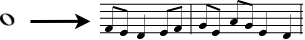
\includegraphics[width=\textwidth,height=\textheight,keepaspectratio]{chapter06/figure-sec1/musicgeneration.png}
        \caption{Sinh nhạc tự động}
    \end{figure}
    
    \item \textbf{Dạng sequence-to-sequence, hay many-to-many bất đối xứng:} 
    
    Dữ liệu đầu vào và đầu ra đều là dạng sequence, tuy nhiên có độ dài khác nhau và không có sự bắt cặp input-output. 
    
    Trong bài toán nhận diện giọng nói, yêu cầu đặt ra là chuyển dữ liệu từ dạng audio sang dạng text. Ta có một sequence đầu vào (audio) và một sequence đầu ra (chuỗi văn bản) với độ dài khác nhau. Bài toán speech recognition được liệt vào dạng sequence-to-sequence.
    
    \begin{figure}[H]
        \centering
        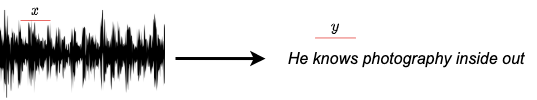
\includegraphics[width=\textwidth,height=\textheight,keepaspectratio]{chapter06/figure-sec1/soundwave.png}
        \caption{Bài toán nhận diện giọng nói}
    \end{figure}
    
    Một ví dụ khác thường gặp là bài toán dịch máy: 
    
    Cho đầu vào là một chuỗi văn bản ở ngôn ngữ A, hệ thống phải trả dữ liệu đầu ra là một chuỗi văn bản ở ngôn ngữ B nào đó. Rõ ràng rằng cũng một câu nói, nhưng ở các ngôn ngữ khác nhau sẽ có cách biểu diễn khác nhau (độ dài câu, số từ, ngữ pháp, ...). Bài toán Machine translation cũng được liệt vào dạng many-to-many bất đối xứng. Cần phân định rõ bài toán dịch máy sequence-to-sequence và word-by-word, word-by-word translation chỉ đơn giản dịch từng từ ở câu cũ và ghép lại thành câu mới.
    
    \begin{figure}[H]
        \centering
        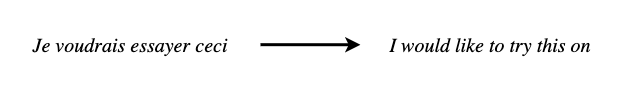
\includegraphics[width=\textwidth,height=\textheight,keepaspectratio]{chapter06/figure-sec1/translation.png}
        \caption{Dịch máy}
    \end{figure}
    
    \item \textbf{Dạng many-to-many đối xứng:} 
    
    Dữ liệu đầu vào và đầu ra đều là dạng sequence, có độ dài như nhau và có sự bắt cặp tương ứng input-output ở từng bước. 
    
    Xét bài toán nhận diện loại từ trong một câu. Vì mỗi từ chỉ thuộc về một loại duy nhất, nên ta sẽ có các cặp input-output đối xứng tương ứng. Hơn nữa, loại từ của một câu cũng phụ thuộc vào các từ đứng xung quanh đó, hay thứ tự xuất hiện của các từ trong câu. Vì vậy, ta liệt bài toán này vào dạng many-to-many đối xứng.
    
    \begin{figure}[H]
        \centering
        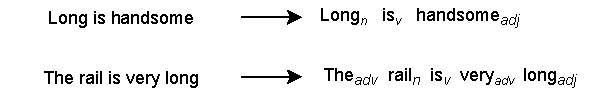
\includegraphics[width=\textwidth,height=\textheight,keepaspectratio]{chapter06/figure-sec1/word_type.pdf}
        \caption{Phân loại từ trong một câu}
    \end{figure}
    \clearpage
    \item \textbf{Dạng many-to-one:} 
    
    Dữ liệu đầu vào dạng sequence, đầu ra dạng cố định. Bài toán phân loại hành động là một trường hợp cụ thể. 
    
    Giả sử, xét đoạn video một người đang đánh golf, input sẽ là sequence nhiều ảnh có thứ tự là từng frame của đoạn videos đó, output kết quả hành động đã đánh golf của vận động viên.
    
    \begin{figure}[H]
        \centering
        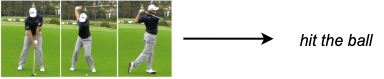
\includegraphics[width=\textwidth,height=\textheight,keepaspectratio]{chapter06/figure-sec1/playgolf.png}
        \caption{Bài toán nhận diện hành động qua video}
    \end{figure}
\end{itemize}

\subsection{Một số vấn đề của mạng neural network thông thường với sequence data}
Các kiến trúc neural network trước (bao gồm MLP và CNN) được xếp vào nhóm feed-forward neural networks. Chúng chỉ đưa ra kết quả dự báo đầu ra chỉ dựa trên dữ liệu đầu vào (không có đường nối vòng trên đồ thị tính toán). Mô hình sẽ hoạt động tốt trong trường hợp giả thiết này là đúng, ví dụ:
\begin{itemize}
    \item Dự báo giới tính của người (đầu ra) chỉ dựa vào ảnh gương mặt của người đó (đầu vào).
    \item Dự báo bệnh ung thư não (đầu ra) chỉ dựa vào ảnh chụp cắt lớp não (đầu vào).
\end{itemize}

Với dữ liệu dạng sequence, đầu ra $y_i$ tại một vị trí bất kì $i$ ngoài bị ảnh hưởng bởi các dữ liệu đầu vào $x_i$, còn có thể bị ảnh hưởng bởi thứ tự xuất hiện của chúng trong sequence. Một số vị dụ cho trường hợp này:
\begin{itemize}
    \item Dự đoán hôm nay trời có mưa hay không? Ngoài việc dựa vào nhiệt độ, độ ẩm, trời nắng/râm, ta cũng có thể dựa vào dữ liệu từ các ngày hôm trước có mưa hay không (có thể xảy ra trường hợp mưa liên tục kéo dài).
    \item Dự đoán giá cổ phiếu cuối phiên giao dịch hôm nay? Giá  có thể dựa vào tình trạng giao dịch, tình hình biến động của thị trường, và lẽ dĩ nhiên cũng dựa vào giá của những ngày hôm trước (giá hôm trước cao kéo theo giá hôm nay cũng cao).
\end{itemize}

Dữ liệu dạng sequence đôi khi còn nằm ở dạng chuỗi dữ liệu thuần túy không dựa trên quan sát:
\begin{itemize}
    \item Dự đoán và đề xuất từ tiếp theo trong chuỗi từ đang nhập từ bàn phím (phổ biến trong bàn phím điện thoại) chỉ dựa vào chuỗi từ đã nhập trước đó.
    \item Dự đoán kết quả sổ xố hôm nay dựa vào kết quả của những ngày hôm trước.
\end{itemize}

Các mạng feed-forward với dạng dữ liệu đầu vào cố định không thể giải quyết bài toán với dữ liệu sequence động (độ dài tùy ý). Tuy nhiên, dữ liệu sequence có thể được biến đổi (tách nhỏ) để sử dụng trên các kiến trúc chỉ dựa vào dữ liệu đầu vào bằng cách lấy một lượng cố định $k$ mẫu các dữ liệu liên tiếp trước đó làm đầu vào. Các model tiếp cận theo hướng này được xếp vào nhóm "auto regressive models". Về tổng quát, một auto regressive model bậc $k$ ($k^{th}$-order) tổng quát có thể được hiểu là một ánh xạ:
\[
    \hat{y}_i = f(x_i, y_{i-1}, y_{i-2},...,y_{i-k})
\]

với $x_i$ là quan sát hiện có, $y_i$ là giá trị sequence ở thời điểm $i$, $\hat{y}_i$ là giá trị dự đoán tại thời điểm $i$, $k$ là bậc của model.
\begin{figure}[h!]
    \centering
    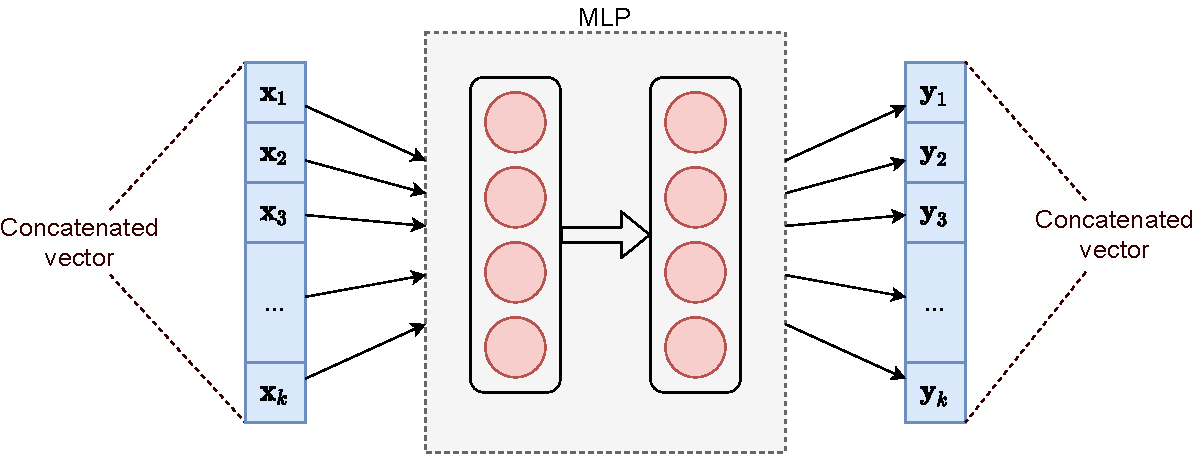
\includegraphics[width=\textwidth,height=\textheight,keepaspectratio]{chapter06/figure-sec1/mlp.pdf}
    \caption{Áp dụng MLP cho bài toán dữ liệu sequence theo dạng regressive model}
\end{figure}

Với hướng tiếp cận như trên, ta tạm thời giải quyết được vấn đề về độ dài dữ liệu bất định. Tuy nhiên, vẫn còn rất nhiều vấn đề khiến MLP không phù hợp cho dữ liệu dạng sequence
\begin{itemize}
    \item Mô hình chưa có khả năng ghi nhớ trạng thái từ các dữ liệu trước đó để hỗ trợ ra quyết định, vẫn phụ thuộc hoàn toàn vào đầu vào. Trong trường hợp cần ghi nhớ dữ liệu ở mức lớn hơn bậc $k$ của mô hình, feed-forward network sẽ không thể đưa ra dự đoán chính xác. Thật vậy, cách mà mô hình regressive model nêu trên lấy dữ liệu từ các mẫu trước đó trong sequence hoàn toàn là do giả định của người thiết kế mạng.
    \item Số lượng tham số là rất lớn: khi sử dụng fully-connected layer, số lượng tham số của một lớp sẽ bằng tích của chiều đầu vào lẫn chiều đầu ra. Lượng tham số lớn sẽ làm ảnh hưởng tới tính chính quy hóa (regularization), khiến mô hình không học hiệu quả mà chỉ overfit trên tập training. Ngoài ra, số lượng tham số quá lớn còn khiến mô hình chiếm rất nhiều tài nguyên cả về bộ nhớ lẫn thời gian huấn luyện.
    \item Mô hình không có khả năng chia sẻ trọng số giữa các bước, ngoài việc sử dụng một lượng lớn tham số dùng riêng cho từng đầu vào. Vì mỗi đầu vào $\textbf x_i$ đều mang tính chất là một điểm dữ liệu trong sequence, ta cần một cách chung tổng quát để xử lý chúng thay vì xử lý mỗi điểm dữ liệu theo một cách riêng (tức phải qua cùng một cách tính toán).
\end{itemize}

Nhắc lại về CNN cho bài toán xử lý ảnh, vấn đề của MLP khi giải quyết bài toán liên quan đến ảnh cũng tương tự như với dữ liệu dạng sequence. Bằng cách thêm giả định (hypothesis) các điểm dữ liệu lân cận sẽ có mối tương quan với nhau nhiều hơn các điểm ở xa (kiến thức thực tiễn từ con người), CNN đã tách việc tính toán trên toàn bộ ảnh thành việc tính toán trên từng vùng cửa sổ nhỏ hơn với cùng một bộ tham số. Tương tự, ở dữ liệu dạng sequence, với giả định thông tin về thứ tự của dữ liệu cũng như cách tính toán trên từng mẫu dữ liệu phải tương đương, người ta đã đưa ra kiến trúc về Recurrent neural network.
